
\documentclass[border=5pt]{standalone}
\usepackage[utf8]{inputenc}
\usepackage[T1]{fontenc}
\usepackage{amsmath,amssymb}
\usepackage{tikz}
\usetikzlibrary{arrows.meta,shapes.misc,calc}
\renewcommand{\familydefault}{\sfdefault}
\tikzset{
  ptcross/.style={cross out,draw,thick,minimum size=1.6mm,inner sep=0pt},
  vec/.style={->,thick,>={Stealth[length=2.6mm]}},
  vecu/.style={vec,color=blue!70!black},
  vecv/.style={vec,color=red!75!black},
  vecw/.style={vec,color=green!45!black},
  grid/.style={gray!35,thin},
}
\newcommand{\Vj}[1]{\overrightarrow{\text{#1}}}
\newcommand{\pt}[4]{\node[ptcross] at (#1,#2) {}; \node[anchor=#4,inner sep=2pt] at (#1,#2) {$#3$};}
\begin{document}
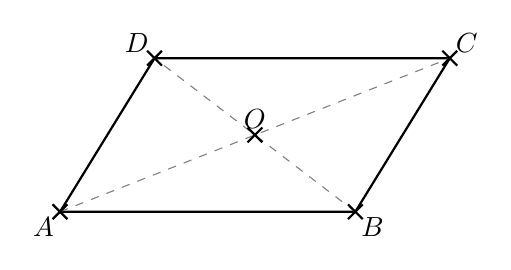
\begin{tikzpicture}[x=0.75cm,y=0.75cm]

\coordinate (A) at (0,0); \coordinate (B) at (5,0); \coordinate (C) at (6.6,2.6); \coordinate (D) at (1.6,2.6);
\coordinate (O) at ($(A)!0.5!(C)$);
\draw[thick] (A) -- (B) -- (C) -- (D) -- cycle;
\draw[gray,dashed] (A) -- (C); \draw[gray,dashed] (B) -- (D);
\pt{0}{0}{A}{north east} \pt{5}{0}{B}{north west} \pt{6.6}{2.6}{C}{south west} \pt{1.6}{2.6}{D}{south east}
\node[ptcross] at (O) {}; \node[anchor=south,inner sep=2pt] at (O) {$O$};

\end{tikzpicture}
\end{document}
